\section{Discretisation}
\label{dis}

Discretization concerns the process of transferring continuous models and equations into discrete counterparts. But whenever continuous data is discretized, there is always some amount of discretization error.

In the field of simulation, a discrete-event simulation (DES), models the operation of a system as a discrete sequence of events in time. Each event occurs at a particular instant in time and marks a change of state in the system.
Continuous simulations contrasts this in the simulation continuously tracks the system dynamics over time. Instead of being event-based, this is called an activity-based simulation; time is broken up into small time slices and the system state is updated according to the set of activities happening in the time slice. The time slices determines the granulity in time.
Another approach is process-based simulation. In this approach, each activity in a system corresponds to a separate process, where a process is typically simulated by a thread in the simulation program. In this case, the discrete events, which are generated by threads, would cause other threads to sleep, wake, and update the system state.

- Something about space granuality, memory and message sizes.

- Number of variables considered in the simulations, is also a granuality.

\subsection{Granuality}
In parallel computing, granularity is a qualitative measure of the ratio of computation to communication. The granualities should be chosen, accordingly with the consideration of this computation / communication ratio. Periods of computation are typically separated from periods of communication by synchronization events.

One can say that \emph{Fine-grain Parallelism is:}
\begin{itemize}
  \item Relatively small amounts of computational work are done between communication events

  \item Low computation to communication ratio

  \item Facilitates load balancing

  \item Implies high communication overhead and less opportunity for performance enhancement

  \item If granularity is too fine it is possible that the overhead required for communications and synchronization between tasks takes longer than the computation.
\end{itemize}
and \emph{Coarse-grain Parallelism is:}
\begin{itemize}
  \item Relatively large amounts of computational work are done between communication/synchronization events

  \item High computation to communication ratio

  \item Implies more opportunity for performance increase

  \item Harder to load balance efficiently
\end{itemize}

\subsection{Decomposition}
  Decompositioning within computer science, is breakinga problem into discrete "chunks" of work that can be distributed to multiple tasks, for the computer to compute.
  In the decompositioning the problem, to multiple task, the designer of the solution can make use of two basic concepts, to partition the tasks in such a way that it can be parallelised, by domain and functional decomposition.

  \emph{Domain decomposition} is distributing similar tasks of a problem among multiple different processors. \cref{dom} illustrates multiple similar tasks that can be parallelised, each working the on their own domain of the problem set.

  \begin{figure}[htbp]
    \label{dom}  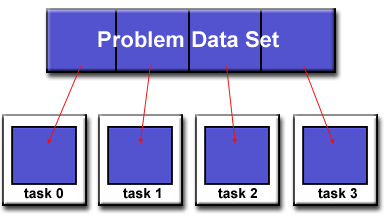
\includegraphics[width=\textwidth]{Analysis/Supercomputing/domain_decomp.png}
    \caption{https://computing.llnl.gov}
  \end{figure}

  This is useful when working with 'for' loops on sets of data, if the operations of each iteration is independent of each other, the loop can easily be split up into multiple parallel tasks.

  \emph{Functional decomposition} focuses on the operations performed rather than on the data manipulated by the computation. Some task differs from other in that they manipulate different data of the problem domain. This is illustrated in \cref{fun}.

  \begin{figure}[htbp]
    \label{fun}  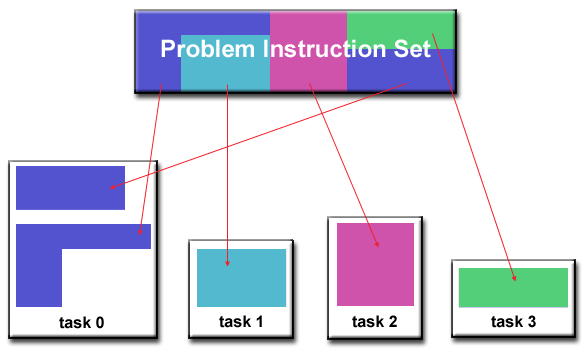
\includegraphics[width=\textwidth]{Analysis/Supercomputing/functional_decomp.png}
    \caption{https://computing.llnl.gov}
  \end{figure}

  This actors with different responsablities in the problem domain
